% D2AI @ IEEE ICDM 2026, DM2158. Camera-ready revision.
% Build: latexmk -pdf -interaction=nonstopmode -halt-on-error main.tex
\documentclass[conference]{IEEEtran}
\usepackage{cite,amsmath,amssymb,amsfonts,booktabs,graphicx,xcolor,url}
\usepackage{algorithm,algorithmic,multirow,array}
\graphicspath{{figures/}}
\IEEEoverridecommandlockouts
\def\BibTeX{{\rm B\kern-.05em{\sc i\kern-.025em b}\kern-.08em\TeX}}

\title{Mining Attention Dynamics:\\Auditing KV-Saliency Prediction in LLMs}
\author{
\IEEEauthorblockN{Ziqing Li}
\IEEEauthorblockA{\textit{Huazhong University of Science and Technology}\\
Wuhan, China \\
d202381502@hust.edu.cn}
\\
\IEEEauthorblockN{Kaicheng Tang}
\IEEEauthorblockA{\textit{The Chinese University of Hong Kong}\\
Hong Kong, China \\
kctang0410@link.cuhk.edu.hk}
\and
\IEEEauthorblockN{Jiawei Guo}
\IEEEauthorblockA{\textit{Beihang University}\\
Beijing, China \\
jwguo@buaa.edu.cn}
\\
\IEEEauthorblockN{Jianxi Chen\thanks{Corresponding author: Jianxi Chen (chenjx@hust.edu.cn).}}
\IEEEauthorblockA{\textit{Huazhong University of Science and Technology}\\
Wuhan, China \\
chenjx@hust.edu.cn}
}
\pdfinfo{/Title (Mining Attention Dynamics: Auditing KV-Saliency Prediction in LLMs) /Author (Ziqing Li, Jiawei Guo, Kaicheng Tang, Jianxi Chen) /Subject (D2AI at IEEE ICDM 2026 - DM2158)}
\begin{document}
\maketitle
\begin{abstract}
Selecting useful key--value (KV) state requires evaluating predictions under the
budget and candidate set of each retention decision. KVSalienceBench audits these
evaluation objects through future-attention labels, explicit selector semantics,
request and source-prompt splits, and versioned collection and validation code.
On corrected traces from two instruction-tuned models, a three-parameter logistic
scorer achieves pooled area under the receiver operating characteristic curve
(AUC) of 0.890, close to LightGBM's 0.896. Yet the within-layer attention signal
recovers 0.659 of each decision's future top-decile blocks, versus 0.613 and 0.615
for those models. This ordering difference narrows at 20\% retention, showing why
pooled ranking and decision-level budgets must be evaluated separately. A separate,
pinned bfloat16 masked-loop rerun over 14 model--dataset cells finds the
runtime-reconstructed scorer and an accumulated-attention baseline equivalent in
mean LongBench F1 within a specified tolerance of two absolute points; both remain
below full-cache quality. Historical served-oracle diagnostics favor the baseline,
but use a different target and experiment version; we audit capacity-forced
misses using logged counts. A feature bridge measures reconstruction effects
without identifying the cause of the historical proxy gap. Reference backends
reduce physical KV storage by about 5.3 times at 20\% retention, with much smaller
reductions in total allocated memory. Extended mask/physical tests produce logit
discrepancies that exceed the preset numerical tolerance. These bounded findings support evaluation alignment,
not a production serving or universal policy-equivalence claim.
\end{abstract}
\begin{IEEEkeywords}
KV cache, attention prediction, empirical audit, calibration, benchmarking,
closed-loop evaluation.
\end{IEEEkeywords}

\section{Introduction}
KV state grows with context while attention concentrates on a subset of
positions. KV-management methods exploit this through
accumulated attention~\cite{h2o}, recent-query observations~\cite{snapkv},
query--key page bounds~\cite{quest}, cross-layer information~\cite{infinigen} and
learned retention~\cite{locret}. Better prediction need not identify a better
retention policy: selection changes later model states and their outputs.
Traceable evaluation of inference state under a budget connects this study to
D2AI's infrastructure, provenance and benchmark scope.

We audit which signals predict future attention, whether predictor complexity
helps, and how proxy rankings relate to answer quality. Offline labels,
served-oracle diagnostics and closed-loop answer scores are distinct objects;
the runtime scorer also reconstructs its features.

\textbf{Contributions.} (1)~\emph{A protocol and benchmark.} KVSalienceBench fixes
future-attention labels, selector semantics (Table~\ref{tab:protocol}), request-
and source-prompt splits, tie-aware per-decision metrics and versioned collection.
(2)~\emph{Controlled findings.} Two attention-magnitude views
support a three-parameter logistic scorer within 0.006 AUC of LightGBM on v2 traces
without a calibration step. At the per-decision top-decile budget, the within-layer
signal recovers more future top-decile blocks than either; this reversal shrinks
at 20\% retention. A separate pinned bfloat16 masked-loop rerun finds
the reconstructed scorer and accumulator mean-F1 equivalent within a pre-specified
$\pm0.02$ margin over 14 model--dataset cells (TOST $p=0.0007$).
A bridge measures feature reconstruction (\S\ref{sec:realization}).
(3)~\emph{An audit and its repair.} We diagnose corrupted float16 Qwen2.5
generation, rerun with a pinned simulator, audit capacity effects from logged counts,
and report physical-KV parity levels. Code, tests and provenance accompany the paper.

\section{Problem and evidence levels}
\label{sec:problem}

\subsection{Attention-defined saliency}
At layer $\ell$ and decode step $t$, let $\mathcal B_{\ell,t}$ contain the logical
KV blocks currently under consideration. A block groups contiguous original token
positions. We aggregate attention by averaging over heads and over a block's token
positions; denote the resulting statistic by $a_{\ell,b,t}$. It is a block-mean
attention statistic, not necessarily a mass normalized to sum to one over blocks.
For a horizon $h$ and a fraction $r$, the target is
$z_{\ell,b,t}^{(h)}=\mathbf 1[b\in\operatorname{Top}_{\lceil r|\mathcal B_{\ell,t}|\rceil}\{a_{\ell,b',t+h}:b'\in\mathcal B_{\ell,t}\}]$:
ranking is restricted to blocks present at $t$. We use $r=0.1$ and horizons
$h\in\{1,4,16,64\}$ (the archived collector's terminal-horizon caveat is in
\S\ref{sec:limits}).

A scorer $f(\mathbf x_{\ell,b,t})$ estimates the label probability from recorded
features; examples arrive in decode order, positives are a small fraction of blocks,
drift is a hypothesis to test, and serial dependence means millions of block rows are
not millions of independent observations.

\subsection{Three different evaluation targets}
Fig.~\ref{fig:paths} locates the evaluation paths.
Offline prediction scores future-attention labels on fixed full-cache traces;
served-oracle diagnostics score a current-attention target along the evaluated
trajectory, and attention importance is not answer correctness; closed-loop task
quality scores answers the selector's own decisions helped produce, here through
masking rather than a cache manager. A fraction of blocks allowed to attend is a
\emph{logical retention budget}, not a fraction of device memory released.

\begin{figure}[t]
\centering
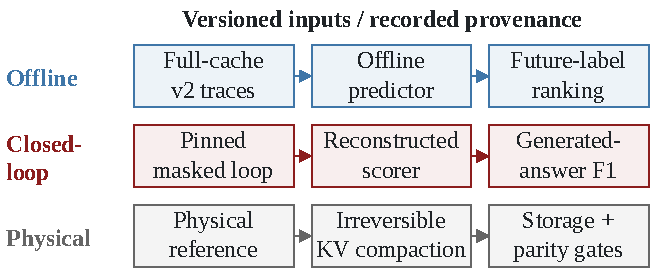
\includegraphics[width=\linewidth]{evaluation_paths.pdf}
\caption{Evaluation paths. Runtime features and selector semantics differ
across paths (Table~\ref{tab:protocol}); physical-reference parity is tested separately.}
\label{fig:paths}
\end{figure}

\subsection{Statistical protocol}
Offline ranking uses AUC, threshold-based AUPRC (tied scores form one group, so
the value cannot depend on row order), precision/recall at $k=r$, Brier score and
expected calibration error (ECE). Top-$k$ metrics are reported pooled over test
rows \emph{and} per cache decision (request, layer, step) at the label's own
$\lceil r\,n\rceil$. Training and testing use disjoint requests and paired
bootstrap intervals resample requests, not block rows. Unless marked otherwise,
intervals are 95\%; equivalence intervals are 90\%. A 10,000-draw sensitivity
analysis jointly resamples all held-out model-requests sharing a source prompt,
on both the original request split and the source-disjoint split.
Top-$k$ score ties use a stable descending sort: pooled ties follow seeded sample
row order, and within-decision ties follow increasing block index. V2 label and
cross-layer indicator boundaries retain the collector's NumPy
\texttt{argpartition} tie rule (implementation-dependent on the original block
order), with exactly $\lceil rn\rceil$ positives; these are not randomized ties.
The main downstream
comparison aggregates paired request scores into architecture--dataset cells and a
TOST analysis~\cite{schuirmann1987tost,lakens2017equivalence} asks whether their
mean difference lies inside a pre-specified margin. Failure to detect a difference
is not equivalence, and equivalence of two comparisons with the same baseline does
not imply equivalence of the remaining pair.

\section{Signals and empirical feature selection}
\label{sec:signals}

\subsection{Recorded views}
The feature family contains a normalized within-layer exponential moving average
(EMA) of attention
$x_{\rm wl}=\bar a_{\ell,b,t}/\max_{b'}\bar a_{\ell,b',t}$, a previous-layer
hot-block indicator $x_{\rm cl}=\mathbf 1[\bar a_{\ell-1,b,t}\text{ is in the top-}r]$,
a query-derived proxy $x_{\rm q}=(1+\cos(\tilde q_t,\tilde K_{\ell,b}))/2$ and a
temporal-age feature $x_{\rm age}=\exp(-(t-p_b)/w)$.
Here $\bar a$ is an EMA and $p_b$ the block-creation step, so $x_{\rm age}$ is an
age proxy, not an LRU access-recency measurement; the tildes mark the archived
query representation, whose coordinate-space audit in \S\ref{sec:limits} limits
conclusions about that view. The cross-layer signal is an attention-magnitude
carry-over, not InfiniGen's query-based mechanism, and the offline extractor falls
back to the current layer's own EMA at layer 0 where runtime realizations need
explicit fallback and alignment rules (Table~\ref{tab:protocol}).

\subsection{Relevance diagnostics}
\label{sec:redundancy}
We estimate relevance $I(X_i;Z)$ with quantile-binned plug-in estimators, in nats.
On the version-2 corpus, within-layer EMA and the cross-layer indicator have $I(X_i;Z)$
of 0.104 and 0.099 nats, versus 0.007 for the cosine query proxy and under 0.001 for age
(\S\ref{sec:exp-relevance}); raw-probe AUCs are in Table~\ref{tab:v2}.

Archived conditional-information diagnostics $U_i=I(X_i;Z\mid X_{-i})$ agree that
the magnitude views carry what the proxies do not ($\le0.006$ nats): within-layer
is $0.133$--$0.155$ on every binning grid and the binary cross-layer estimate
$0.048$--$0.084$ on the finer ones, collapsing to zero under the coarsest, so the
artifact reports its grid sensitivity. These estimates motivate a candidate subset,
evaluated on held-out requests; they are not a sufficiency certificate, and the
evidence for the compact model is its measured predictive performance.

\section{Predictor family and feature realizations}
\label{sec:method}

\subsection{A compact offline scorer}
We fit a ridge-regularized logistic model by Newton--IRLS,
$f(\mathbf x)=\sigma(\mathbf w^\top\mathbf x+b)$; on the within-layer and
cross-layer features it has two coefficients and one intercept. A
log-loss fit without class reweighting has low measured ECE here and the
class-balanced LightGBM does not, but an unweighted or recalibrated tree removes
that difference (\S\ref{sec:exp}): calibration is separate from ranking here.

\subsection{Offline predictor versus runtime reconstruction}
\label{sec:realization}
The masking-loop scorer reconstructs the cross-layer view from the previous
layer's EMA, neutralizes the query view, and feeds selection into later states, so
its task F1 cannot inherit the offline predictor's AUC. Table~\ref{tab:protocol}
distinguishes fixed offline features, policy-dependent runtime features and the
irreversible physical reference.
\textbf{Bridge experiment.} With the frozen archived two-view checkpoint, one label
(top-$\lceil0.1n\rceil$ of block attention four steps ahead among the blocks present
now and still present then) and the 128 frozen prompts of \S\ref{sec:deploy}, we
score (A) offline-style features re-derived from the full-cache attention stream under
version-2 conventions, (B) the reference backend's runtime realization on the same
rows, and (C) that realization along the on-policy trajectory at 20\% budget. In A and B the candidates are every block present; in C they are the blocks
retained now \emph{and} at $t+h$, a survivor-conditioned arm whose $n$ and label
denominator are taken among those survivors. Mean per-request AUC is
0.902/0.899/0.989 on Llama-3.1-8B (bfloat16) and 0.894/0.892/0.989 on Qwen2.5-7B
(float32): the feature realization costs $-0.003$ $[-0.004,-0.001]$ (84/128
requests negative) and $-0.002$ $[-0.003,-0.000]$ (75/128), whereas the on-policy
arm is higher by $+0.090$ and $+0.098$ (128/128 both). That is not evidence that
retention makes prediction easier: C ranks only blocks the policy already kept, so
an evicted block can never be missed, and the value neither isolates a feedback
effect nor measures the coverage lost to eviction. Neither contrast reproduces the
archived 0.948-to-0.643 drop of \S\ref{sec:historical}, which also differs in
corpus, aggregation and numerics; attribution would need a label-only arm on
identical trajectories, candidates, features and scorer, so that gap stays
unexplained.

\subsection{Selector semantics across the three evidence objects}
\label{sec:protocol}
Table~\ref{tab:protocol} lists the rules that decide what each object measures. Two
differ on purpose: the masked loop (pinned-rerun rules) recomputes its kept set every
eight steps, so an
excluded block can return, and budgets $\mathrm{round}(0.2n)$ blocks with $n$
counting the blocks of generated tokens too, whereas the reference deletes
irreversibly and fixes its budget from the prompt.

\begin{table}[t]
\centering
\caption{Selector and label semantics. Blocks are 32 tokens; $n$ is the candidate
count, $L$ the prompt length, $K$ the oracle size of Exp\#7. The loop's budget wins when
it is below its mandatory set (7 blocks on one prompt per model).}
\label{tab:protocol}
\footnotesize
\setlength{\tabcolsep}{2.5pt}
\begin{tabular}{@{}>{\raggedright\arraybackslash}p{0.17\columnwidth}>{\raggedright\arraybackslash}p{0.26\columnwidth}>{\raggedright\arraybackslash}p{0.26\columnwidth}>{\raggedright\arraybackslash}p{0.22\columnwidth}@{}}
\toprule
rule & v2 collector & masked loop & physical reference \\
\midrule
attention & head/token mean; ragged block over members & head-group/query mean; ragged block padded & head/query/token mean \\
EMA & decay 0.9 from first decode value & H2O-style: last-32 sum; reconstructed: last-8 EMA, 0.9 & decay 0.9; last-64 prefill queries \\
within view & $\bar a/(\max\bar a+10^{-9})$ & $\bar a/(\max\bar a+10^{-9})$ & $\bar a/\max\bar a$ \\
cross view & previous-layer EMA top-$\lceil0.1n\rceil$; layer 0: own EMA & same rank rule; layer 0: own EMA & same rank rule; layer 0: zero \\
query / age & post-RoPE $q$; age from block creation & query 0.5; age since last top-$k$ & unused \\
label & future top-$\lceil0.1n\rceil$, real lookahead & current unmasked top-$K$ (Exp\#7) & unused \\
budget & --- & round$(0.2n)$, every 8 steps & $\lfloor0.2\lceil L/32\rceil\rfloor$, prompt-fixed \\
mandatory & --- & reconstructed: 4 sink~\cite{streamingllm} + 4 recent; H2O-style: half heavy, half recent & 1 sink + 1 recent \\
re-admission, new tokens & --- & allowed at each decision; new tokens unmasked, budget grows & irreversible; new tokens eligible, fixed budget \\
\bottomrule
\end{tabular}
\end{table}

\subsection{Thresholds and online updates}
\label{sec:online}\label{sec:conformal}
A score can drive a fixed-size top-$k$ set or a thresholded set
$S_{\ell,t}=\{b:f(\mathbf x_{\ell,b,t})\ge\tau_\ell\}$. The former fixes logical
retention, whereas the latter lets set size vary. We evaluate static and online
variants separately. Threshold results are reported in \S\ref{sec:guardkv};
its empirical in-distribution performance is not a hard per-request risk guarantee.

\section{Prediction measurements}
\label{sec:exp}

\textbf{Data and comparators.} Corrected version-2 traces carry the offline
evidence; version-1 diagnostics are in \S\ref{sec:historical}. Single-signal rows
score one recorded feature and do not reimplement the papers that motivate them;
the learned comparators are LightGBM on all four views (150 trees of depth 3) and the
two-view logistic fit, with larger logistic, MLP and online fits left to the
artifact. Every fit, including the isotonic
control's calibration split, uses held-in requests only, and no held-out request
enters a fit or a threshold; the two-view subset was fixed from version-1
diagnostics, so the version-2 relevance estimates below are descriptive.

\subsection{Exp\#1: Ranking and calibration}
\label{sec:exp-relevance}
\textbf{Version-2 corpus.} Table~\ref{tab:v2} uses checksum-verified traces of the same
128 LongBench QA prompts (64 Qasper, 64 NarrativeQA) for Llama-3.1-8B and Qwen2.5-7B:
30.4M rows and 256 model-requests. Pooled metrics use 120K training and 150K held-out
rows; per-decision metrics use every held-out row. Refitting both models on the same split, seed and test rows at up to all 22.8M held-in
rows (190-fold) lifts LightGBM by 0.0005 AUC (0.8961 to 0.8966), widens the paired
deficit only from $-0.0057$ to $-0.0062$ $[-0.0073,-0.0051]$, and its per-decision recall
holds at 0.615, so the gap is stable to training size; six LightGBM capacities (depth
3--8, 150--600 trees, one leaf-limited, balanced or not) at 120K and 1.92M rows keep its AUC lead between
0.0005 and 0.0076 and its per-decision recall between 0.615 and 0.622, never reaching
the raw EMA's 0.659. The split holds out 64 model-requests, so Table~\ref{tab:v2}
measures transfer to new model-requests, not to unseen text: 50 of their 57 source
prompts also occur in training through the other model. A source-disjoint split (the
same 32 prompts held out for both models; the benchmark's default) agrees within 0.006
AUC for every method and reproduces every entry of the lower block within 0.004
(top-decile recall 0.656, 0.610 and 0.612). The two-view fit reaches AUC 0.890 (source-prompt bootstrap
$[0.882,0.898]$) against LightGBM's 0.896, a paired deficit of $-0.0057$
$[-0.0068,-0.0046]$, larger than the version-1 $-0.0010$ but still small. At the
per-decision operating point the ordering changes: the raw within-layer EMA
recovers 0.659 of each decision's future top-decile blocks against 0.613 for the two-view
fit and 0.615 for LightGBM, though its pooled top-decile precision (0.542) and AUC
(0.873) are lower. The decision-macro gaps are $+0.046$ $[0.042,0.049]$ and $+0.044$
$[0.041,0.047]$ (source-cluster bootstrap of the decision-macro statistic, 10,000 joint
draws of 57 source prompts), and $+0.046$ $[0.043,0.049]$ and $+0.045$ $[0.042,0.048]$ on
the source-disjoint split; the gap is positive within each of the 64 held-out requests
on both, and the ordering holds in each model (recall 0.652, 0.616 and 0.616 on Llama;
0.665, 0.610 and 0.614 on Qwen). The reversal's size depends on the operating point: at
the closed loop's 20\% budget, per-decision recall is 0.840, 0.838 and 0.830 and the gaps
fall to $+0.002$ $[0.002,0.003]$ (positive in 52/64 requests) and $+0.010$
$[0.009,0.011]$, consistent with, but not explaining, Exp\#8's mean-F1 equivalence.

\textbf{Where the reversal comes from.} Within one decision the within-layer view is a
monotone rescaling of the raw EMA (its denominator $\max_{b'}\bar a_{\ell,b',t}$ is shared
by the candidates), so $\sigma(w_1x_{\rm wl}+w_2x_{\rm cl}+b)$ reorders the raw view
through exactly one term, the \emph{binary} cross-layer indicator: a fixed offset
$w_2/w_1=0.025$ ($w_1=97.7$, $w_2=2.46$) against a corpus mean $x_{\rm wl}$ of 0.015. The
lower block of Table~\ref{tab:v2} evaluates Eq.~(\ref{eq:split}) on every held-out row.
Its weight $\omega$ depends on the decision sizes, not on the scorer: 0.0016\% here,
about one over the 61,184 decisions. That pooled AUC is a cross-decision statistic is
therefore arithmetic; the finding is what one fitted term does to the two parts. The
indicator raises pooled AUC by $+0.017$ $[0.015,0.019]$ but lowers pair-weighted
within-decision AUC by 0.0025 $[0.0023,0.0028]$ and top-decile recall by 0.046;
scaling the offset by $\lambda$ (Fig.~\ref{fig:redundcalib}(a); $\lambda=0$ is the raw
EMA order, $\lambda=1$ the fit) shows one eighth of the offset already gives 83\% of
the first and 65\% of the second. At the top-decile boundary the term swaps in 22\% of the
selected blocks, all previous-layer-hot: 20\% are positive, against 41\% of the blocks
they displace. The indicator is informative overall (61\% of previous-layer-hot blocks
are future top-decile blocks, 4\% of the rest) but not at the margin; every decision
holds exactly $\lceil0.1n\rceil$ positives, so it cannot be flagging salient-rich
decisions, and why it makes scores comparable across decisions is untested. LightGBM
moves the same way ($+0.022$ pooled AUC, $-0.005$ within-decision AUC, $-0.044$ recall).

Relevance and reliability: the magnitude views carry $I(X_i;Z)$ of 0.104 and 0.099 nats,
the query proxies 0.007 (cosine) and 0.025 (dot-max), the age proxy under 0.001, on a
400K-row sample of all pooled rows (from held-in rows only they move by at most 0.0011).
The class-balanced LightGBM has ECE 0.208 (Fig.~\ref{fig:redundcalib}(b)) while the
unweighted (0.005) and isotonic (0.003) variants match the two-view fit (0.006). The
isotonic control reserves 48 of the 192 training model-requests, its trees use the other
144, and the 64 test requests are excluded from both fitting stages: request-level
calibration separation, not source-level independence.

\begin{figure}[t]
\centering
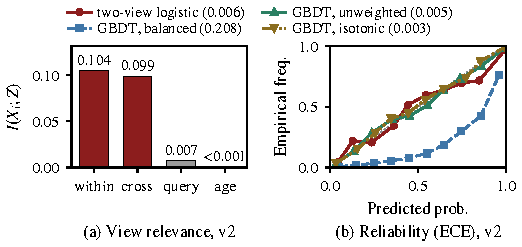
\includegraphics[width=\linewidth]{fig_redund_calib.pdf}
\caption{Exp\#1, version-2 corpus. (a) The fitted cross-layer offset scaled by $\lambda$
from 0 (raw within-layer EMA order) through 1 (the fit) to 2, on every held-out row: pooled
AUC and per-decision top-decile recall as changes from the raw EMA. (b) Reliability of the two-view fit and
of class-balanced, unweighted and isotonic LightGBM in 10 equal-width bins; ECE in
parentheses.}
\label{fig:redundcalib}
\end{figure}

\begin{table}[t]
\centering
\caption{Exp\#1: version-2 ranking and calibration, horizon 4, request split.}
\label{tab:v2}\label{tab:main}
\footnotesize
\setlength{\tabcolsep}{2pt}
\begin{tabular*}{\columnwidth}{@{\extracolsep{\fill}}lccccc@{}}
\toprule
method & AUC & AP & P@$k$ pool & P@$k$ dec. & ECE \\
\midrule
%%V2-ROWS-BEGIN%%
age proxy & .502 & .102 & .102 & .109$^{\dagger}$ & --- \\
query proxy (cosine) & .599 & .135 & .147 & .415 & --- \\
prev-layer indicator & .783 & .412 & .609 & .610 & --- \\
within-layer EMA & .873 & .609 & .542 & .659 & --- \\
LightGBM, balanced & .896 & .674 & .626 & .615 & .208 \\
two-view logistic, refit & .890 & .667 & .624 & .613 & .006 \\
two-view, archived weights & .890 & .667 & .622 & .611 & .019 \\
%%V2-ROWS-END%%
\midrule
method & pooled & within & cross & rec.\,10\% & rec.\,20\% \\
\midrule
%%DEC-ROWS-BEGIN%%
within-layer EMA & .873 & .930 & .873 & .659 & .840 \\
two-view logistic, refit & .890 & .928 & .890 & .613 & .838 \\
LightGBM, balanced & .895 & .925 & .895 & .615 & .830 \\
%%DEC-ROWS-END%%
\bottomrule
\end{tabular*}
\par\smallskip
\begin{minipage}{\columnwidth}\footnotesize
Upper block, 150K sampled held-out rows: AP is tie-aware AUPRC; ECE only for
probability outputs; P@$k$ dec.\ is top-decile precision (equal to recall there),
decision-macro over the 61,184 decisions of all 7.6M held-out rows.
$^{\dagger}$Expectation under random tie-breaking (.208 by row order,
\S\ref{sec:problem}). Lower block, every held-out row (LightGBM .895 pooled against
.896 on the sample): pair-weighted AUC over within- and cross-decision pairs
(Eq.~(\ref{eq:split})); decision-macro recall. Further rows are in the artifact.
\end{minipage}
\end{table}

\section{An empirical risk-target construction}
\label{sec:guardkv}
\textbf{Exp\#4: Risk-target calibration.} GuardKV maps a target miss rate to a
per-layer threshold calibrated on held-out requests; in the archived
in-distribution test, measured miss tracks the target within 0.007 and targets of
0.05 and 0.20 yield retention near 34\% and 14\%. The rule is explicit: with $s_{\ell,(1)}\le\dots\le s_{\ell,(n_\ell)}$ the sorted
scores of layer $\ell$'s $n_\ell$ salient calibration rows, the threshold for target
miss $\alpha$ is $\tau_\ell=s_{\ell,(k)}$, with
$k=\min(n_\ell,\lfloor\alpha(n_\ell+1)\rfloor)$ and the sentinel
$s_{\ell,(0)}=0$; an empty pooled positive set also gives threshold zero.
Layers with under 64 salient rows use the pooled threshold, and the retained set is
$\{b:p_b\ge\tau_\ell\}$ plus four sink and four most-recent blocks. This
corrected implementation uses one-based ranks; the archived helper indexed the
same rank from zero, one order statistic higher. The quoted historical results
are unchanged empirical measurements, not verification of the corrected rule.
The split-conformal quantile has finite-sample marginal coverage only under
exchangeability of calibration and test units, not established for correlated
block/step rows, and marginal coverage would not imply a per-request bound; against
the served-oracle target the reconstructed scorer needs about full retention for
90\% coverage, and no out-of-distribution, hard-budget or production-risk guarantee
is made.

\section{Runtime scope and scoring cost}
\label{sec:deploy}

\textbf{Masking is not physical eviction.} The closed-loop experiments exclude
selected blocks from attention and score generated answers; equal outputs under
physical eviction would need matched token histories, kept sets, position
semantics, feature availability and re-admission rules, none of which the simulator
establishes, so its task-quality result is scoped to the masked loop and is not a
serving claim (\S\ref{sec:limits}). \textbf{Exp\#5: Scoring-only cost.} The archived microbenchmark times 28.7\,$\mu$s
at P99.9 for one 4096-vector batch of the four-weight kernel; it excludes feature
extraction, selection and compaction and is not a serving TPOT.

\textbf{Exp\#6: Physical-KV implementation check.} We evaluate an eager,
single-request reference backend with original token positions, irreversible block
eligibility and independent compact K/V storage, against a dense masked reference
under the same eligibility rule (Table~\ref{tab:protocol}). Gates compare native
full-cache logits with the no-eviction path and replay a frozen teacher schedule
between mask and compact storage. \texttt{h2o\_block} is a shared-head block
accumulator, not a reproduction of H2O or Ada-KV, and the runner implements no
paging, offload, batching or production throughput.

Table~\ref{tab:physical} reports both models on one A100-80GB, Transformers 4.51.3,
greedy decoding, the same 128 English QA prompts (64 Qasper, 64 NarrativeQA), input
cap 4096, at most 128 new tokens and middle truncation on 104/128 prompts.
Llama-3.1-8B-Instruct runs in bfloat16; Qwen2.5-7B bfloat16 parity exceeded the
preset tolerance (maximum absolute error 0.25 versus 0.15) while argmax agreed, so
Qwen is reported in float32. At 20\% budget compact storage equals the live payload
whereas the mask keeps full-size tensors, a $5.3\times$ ratio for both. Greedy
sequences match between the two paths on 98/128 and 100/128 Llama requests (mean
absolute F1 differences 0.014 and 0.007) and 128/128 Qwen requests. Allocator decode
peaks fall only from 15.51 to 15.10\,GiB (Llama) and 29.05 to 28.63\,GiB (Qwen)
because weights dominate, with prefill-plus-first-compaction peaks at 15.77 and
29.23\,GiB. Two task clusters are too few for reliable cross-task equivalence
inference; the 30\% cells
are in the artifact, and gates at the full input with 40 decode steps are in
\S\ref{sec:limits}.

\begin{table}[t]
\centering
\caption{Exp\#6 (Physical-KV check) at 20\% block budget. Stored KV is mean unique
K/V tensor storage (MiB) after the last step, live KV the mean retained payload,
ITL (ms) the median local inter-token latency, not a request-level serving TPOT.
Llama bfloat16, Qwen float32.}
\label{tab:physical}
\begin{tabular*}{\columnwidth}{@{\extracolsep{\fill}}llcccc@{}}
\toprule
model & realization & F1 & stored & live & ITL \\
\midrule
Llama & full physical & .223 & 496 & 496 & 76.1 \\
 & H2O-style mask & .183 & 496 & 94 & 61.0 \\
 & H2O-style physical & .181 & 94 & 94 & 56.9 \\
 & reconstructed mask & .177 & 496 & 94 & 60.0 \\
 & reconstructed physical & .178 & 94 & 94 & 57.9 \\
\midrule
Qwen & full physical & .246 & 434 & 434 & 71.4 \\
 & H2O-style mask & .233 & 434 & 82 & 58.2 \\
 & H2O-style physical & .233 & 82 & 82 & 54.4 \\
 & reconstructed mask & .232 & 434 & 82 & 58.1 \\
 & reconstructed physical & .232 & 82 & 82 & 54.4 \\
\bottomrule
\end{tabular*}
\end{table}

\section{Closed-loop task quality}
\label{sec:transfer-gap}

\textbf{Exp\#8: Matched-retention answer quality.}
The policy evaluated here is the runtime reconstruction of
\S\ref{sec:realization}, not the offline predictor of Table~\ref{tab:v2}. The main
comparison uses chat-formatted LongBench QA~\cite{longbench}: its seven English
question-answering datasets (NarrativeQA, Qasper, MultiFieldQA-en, HotpotQA,
2WikiMultihopQA, MuSiQue, TriviaQA; abbreviated in Fig.~\ref{fig:forest}), two
architectures (Llama-3.1-8B and Qwen2.5-7B) and 448 source prompts, 64 per dataset, each
evaluated on both architectures (896 model--prompt evaluations, 64 per
architecture--dataset cell), at 20\% logical retention, each policy driving its own
masked decoding trajectory.

\textbf{Inferential unit and margin.} Because the two architectures answer the same
questions, the 14 cells are not independent. The primary analysis averages the two
models within each dataset and runs paired TOST over the seven datasets (df 6); the
14 cells treated as independent are a sensitivity analysis. The margin is two
absolute F1 points, 5.4\% of the rerun baseline 0.372: a practical tolerance carried
over from the archived analysis, not pre-registered and not a deployment threshold.
Fig.~\ref{fig:forest} exposes task heterogeneity: mean equivalence is not per-task.

\begin{figure}[t]
\centering
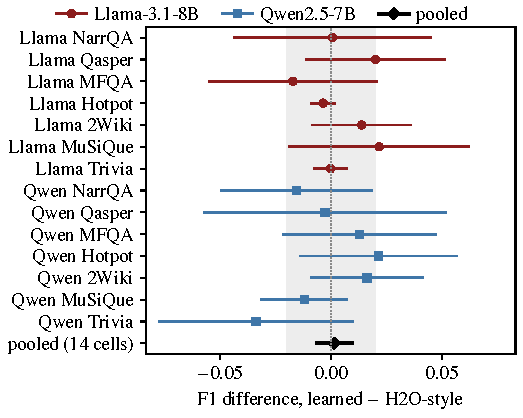
\includegraphics[width=\linewidth]{fig_cell_forest.pdf}
\caption{Exp\#8, pinned bfloat16 rerun. Reconstructed-minus-H2O-style F1 per
architecture $\times$ dataset cell (64 paired requests, 95\% t intervals; the two models
of a dataset adjacent) and pooled estimates (90\% t intervals): seven datasets (primary,
filled) and 14 cells (sensitivity, hollow); the band is the $\pm0.02$ margin.}
\label{fig:forest}
\end{figure}

\begin{table}[t]
\centering
\caption{Exp\#8: masked-loop LongBench F1 at 20\% retention, 896 model--prompt
evaluations. $\Delta$ is the difference from the H2O-style accumulator with a 90\% $t$
interval over the seven datasets (df 6); $p_{\mathrm{TOST}}$ is the TOST $p$ at
$\pm.02$ over the same datasets. Pinned bfloat16 rerun, official scorer, all
references.}
\label{tab:perlayer}
\footnotesize
\setlength{\tabcolsep}{3pt}
\begin{tabular*}{\columnwidth}{@{\extracolsep{\fill}}lccc@{}}
\toprule
policy realization & F1 & $\Delta$ [90\% CI] & $p_{\mathrm{TOST}}$ \\
\midrule
%%PERLAYER-ROWS-BEGIN%%
full cache & .419 & +.047 & --- \\
H2O-style & .372 & --- & --- \\
reconstructed & .374 & +.002 [-.006, +.010] & .0023 \\
Ada-KV-style & .363 & -.008 [-.016, -.000] & .015 \\
PyramidKV-style & .349 & -.023 [-.046, +.001] & .582 \\
%%PERLAYER-ROWS-END%%
\bottomrule
\end{tabular*}
\end{table}

\textbf{Pinned rerun.} With the official LongBench scorer and all references, the
reconstructed scorer's mean F1 difference from the accumulator over 896 evaluations is
$+0.0017$: the seven-dataset TOST gives $p=0.0023$ at $\pm0.02$ and the 14-cell
sensitivity analysis $p=0.0007$. The seven-dataset $t$ interval is $[-0.0064,0.0098]$;
the 14-cell $t$-based and cell-bootstrap 90\% intervals are $[-0.0063,0.0097]$ and
$[-0.0056,0.0087]$. Supplementary $\pm0.01$ tests ($p=0.047$ seven datasets, 0.045 14 cells) use a margin
that was not set in advance, so we do not count them. Per architecture the
difference is $+0.0052$ (Llama, $p=0.016$) and $-0.0018$ (Qwen, $p=0.026$). The
Ada-KV-style comparator remains equivalent ($-0.0084$, $p=0.015$); the PyramidKV-style
one does not ($-0.023$, $p=0.58$). Both allocation comparators only move a fixed total
budget across layers (Ada-KV-style: by attention concentration; PyramidKV-style: a
linear pyramid) and select within a layer as H2O-style does, so no finding covers original H2O, Ada-KV or
PyramidKV, or equivalence between the reconstructed and Ada-KV-style policies; and this
is equivalence between compressed policies, not absence of compression loss: both stay
0.045--0.047 below full cache. The policies also differ in EMA window and mandatory
blocks (Table~\ref{tab:protocol}): this compares two complete runtime realizations, not
a scorer-only intervention, which is untested. Logged retained blocks per decode step
average 25.02 for the H2O-style, reconstructed and Ada-KV-style policies and 25.01 for
the PyramidKV-style one (median 26, range 7--26): retention is matched in counts, not
only in the nominal 0.2.

\textbf{What the rerun repaired.} Archived Qwen float16 decoding emitted all-NaN logit
rows, producing token~0 (``!''): a 56-prompt replay found this in 54 requests, against
none in bfloat16/float32. In the rerun no Qwen
full-cache output contains a run of ``!'' (0/448 versus 181/448) and 34/448 reach the
48-token cap (versus 210/448). The archived F1 difference was $+0.00511$ under a
single-reference scorer ($+0.0030$ after all-reference rescoring); the artifact keeps
the original scores and the repair record.

\textbf{Exp\#9: Archived budget and context checks.} Sweeping retention over
$\{0.10,0.20,0.30,0.50\}$ yields no resolved per-budget quality gain; at 16K the larger
Llama sample (448 prompts, 20\% retention) has mean F1 difference $-0.0006$,
request-level 95\% interval $[-0.012,0.012]$, and a 160-prompt pilot that had suggested
$+0.010$ is not sustained, so we claim no long-context gain. A synthetic needle
probe is a negative control, not evidence about query-aware selection. Neither check
proves curve equivalence or zero memory saving.

\section{Limitations and artifact audit}
\label{sec:limits}

\textbf{External validity.} Historical traces cover four instruction-tuned 7--8B
families; corrected v2 traces and the pinned task-quality rerun cover two, at up
to about 4K context. The archived 16K Llama and short-context Qwen2.5-14B runs are
separate checks, not v2 replications (14B F1 0.301/0.307/0.301
for accumulator, reconstructed scorer and adaptive-allocation comparator); nothing
is extrapolated to MoE, base checkpoints, 32K contexts or sampling, and decoding is
greedy.

\textbf{Query-coordinate audit.} The legacy extractor hooks \texttt{q\_proj} before
rotary transformation but reads post-rotation keys, so it never computed the
attention-space query--key product, and its revision is unpinned; we withdraw the
``faithful Quest'' reading of the old dot-max probe and claim no intrinsic query
redundancy. Version 2 aligns queries and keys after RoPE, with a one-head test that
its scaled dot products reproduce the model's attention probabilities; even so a
dot-max probe is not Quest's page-bound algorithm. Adding it to the two magnitude
views changes held-out \emph{request-mean} AUC by $-0.0070$ on the 128 Llama prompts
(32 test requests, all negative; $[-0.0082,-0.0058]$; two-view mean 0.899) and by
$+0.0020$ on the matched Qwen prompts (31/32 positive; $[0.0016,0.0024]$; mean
0.884): small, model-dependent changes with opposite signs in the two tested
configurations, which the pooled
version-2 value averages away. Some legacy long-context drivers also disabled
prefill attention, depriving query-aware selectors of observations while leaving
accumulators usable, so neither those comparisons nor the needle probe rank faithful
query-aware implementations.

\textbf{Generation and label boundaries.} The legacy collector refed the final
prompt token to start decode and clamped unavailable horizons to the last recorded
step; version 2 consumes the prefill-predicted token and generates genuine lookahead.
No archived number was silently replaced, and the archived horizon curve is not
evidence for long-horizon generalization.

\textbf{Generation path and scorer of the archived loop.} The archived cells came
from an unpinned simulator in float16, whose Qwen2.5 path emits all-NaN logit rows
(\S\ref{sec:transfer-gap}), scored against one reference with articles removed
before punctuation. The rerun pins the revision by hash, uses bfloat16 for both
architectures and applies one memory patch (a placeholder replaces each layer's
already-ingested attention weights in the tuple returned to the decoder layer;
verified on a tiny model to change no statistic, mask or token). No rerun latency is
reported; the GPUs were shared.

\textbf{Tied scores and shared prompts.} The archived AUPRC integrated one row at a
time after a stable sort, crediting tied scores for row order; the two discrete
probes are affected and cannot be recomputed, since the version-1 rows are gone, so
Table~\ref{tab:v2} uses the threshold-based definition. The four archived families
shared 32 prompts, so the archived split holds out model-requests, not source texts;
version 2 adds a source-prompt split.

\textbf{Inference and calibration.} Block-level information estimates depend on
binning and conditional sparsity; overlapping marginal intervals are not an
equivalence test; the main TOST treats cell means as independent units, so its
conclusions hold for this fixed collection of two architectures and seven tasks,
exploratory samples are not replications of it, and non-rejection does not establish
no benefit.

\textbf{Parity levels of the reference backend.} The committed gates (1024 tokens,
four decode steps) pass their numeric tolerance. Extending them to four prompts from
both datasets, 1024--4096 input tokens and 40 decode steps with repeated eviction
separates three levels: the session reproduces native full-cache logits exactly
(maximum error 0 in all 12 runs); the compact and masked paths, fed the same teacher
tokens and schedules, drift apart over successive evictions to a maximum logit
difference of 0.66--1.44 in bfloat16 (3.5--5.9$\times$ the preset tolerance) and
$3.6\times10^{-5}$--$1.9\times10^{-4}$ in float32 (1.3--6.1$\times$), so the
extended test fails its preset tolerance. That the difference falls by four orders
of magnitude with precision is consistent with floating-point ordering accumulated
over 40 evictions, but these runs do not exclude a semantic difference; settling it
needs a layer-by-layer comparison of retained indices, absolute positions and K/V
values against a higher-precision reference. Top-1 agreement is 972/984 gated steps in bfloat16 and
984/984 in float32; free-running greedy parity is 98--100/128 (Llama) and 128/128
(Qwen). Tolerances were not raised; the records are in the artifact.

\textbf{System boundary.} The old physical-memory probe swallowed decode
exceptions, put full prefill in its peak statistic and had no verified
absolute-position or repeated-eviction protocol; it is retired, its source and
results kept for provenance. Scoring microseconds, kept-set sizes and synthetic
latency components measure none of production TPOT, HBM release, contention or
throughput.

\textbf{Availability.} The artifact contains LaTeX, result JSON, analysis code,
predictor weights, tests, the version-2 collector and the reference validator. The
rerun's exact simulator source is bundled with its MIT notice and verified against
all 70 cells' provenance hashes. A CPU example, environment and data/model
preparation instructions accompany it; model weights remain separately licensed.
Code, records and figure sources are at
\url{https://github.com/lzbaclz/KVSalienceBench}; raw traces are available by request.

\section{Related work}
\label{sec:related}
Streaming learning studies evolving examples and distribution
shift~\cite{gama2014drift}; multi-view learning and relevance--redundancy analysis
motivate comparing information sources~\cite{blummitchell,peng2005mrmr}, which we
apply to recorded attention dynamics without treating a small information estimate
as a sufficiency proof. Our pooled-versus-within-decision split parallels
user-weighted (grouped) AUC in click-through prediction~\cite{zhou2018din}, which
averages per-user AUC by impressions because pooled AUC also rewards cross-user order;
Eq.~(\ref{eq:split}) weights by pairs instead.
Calibration and conformal
prediction~\cite{guo2017calibration,angelopoulos2023gentle,gibbs2021aci} provide
tools whose guarantees do not transfer to dependent runtime observations unchecked.

KV-management methods use heavy hitters, attention sinks with recent windows,
recent observations, cross-layer signals, query bounds, adaptive allocation and
learned retention~\cite{h2o,streamingllm,snapkv,quest,infinigen,adakv,pyramidkv,locret};
PagedAttention~\cite{pagedattention} addresses physical serving. Our probes and
allocation comparators are not interchangeable with those systems; this is an audit of
the links between intermediate prediction and task quality, not a claim that these
methods are unnecessary.

Closest to our question are prediction-first methods and evaluation suites for KV
compression. AttentionPredictor~\cite{attentionpredictor} learns a lightweight
model of next-token attention and uses it to identify critical tokens; we do not
compare against it and ask instead which evaluation link a proxy's ranking survives.
Gao et al.~\cite{gao2025rethinking} audit compression from the
serving side, and Agrawal and Mayer~\cite{agrawal2026benchmarking}
benchmark task quality, throughput, time-to-first-token and compression ratio
jointly. SCBench~\cite{scbench} evaluates the whole KV-cache lifecycle, including
shared-context reuse, and reports attention-distribution shift in long generation.
Expected Attention~\cite{kvpress} scores each KV pair by the attention expected from a
distribution of future queries, itself a prediction of future attention, and releases
KVPress, which standardizes more than twenty compression methods;
KVzap~\cite{jegou2026kvzap} is a recent learned pruning method evaluated on such a
suite, and Locret~\cite{locret} trains retaining heads on a causal-importance target
and validates them by end-task quality. Those suites and task-level benchmarks such
as LongBench and RULER~\cite{longbench,ruler} fix a common harness and ask whether a
method is worth deploying; we fix the scorer and the label and vary the feature
realization and the candidate set (\S\ref{sec:realization}, Exp\#7--8). The negative findings concern how proxies
transfer to task quality in the tested implementations, not the value of learned or
value-dependent selection~\cite{vatp}.

\section{Conclusion}
KV-saliency prediction and KV retention are related but distinct evaluation
problems. On version-2 traces, the ranking advantage of learned scorers in pooled
metrics reverses under per-decision top-decile budgets and narrows at 20\%
retention. A separate pinned bfloat16 masked-loop rerun finds the reconstructed
scorer mean-F1 equivalent to an accumulator within $\pm0.02$, while both lose
quality relative to full cache. Historical served-oracle diagnostics favor the
accumulator; they are not a same-version proxy--quality experiment. The bridge
quantifies feature reconstruction at $-0.003$ AUC, but jointly changing trajectory
and candidates does not explain the archived gap; a label-only arm is still missing.
These findings concern the tested data and implementations, not the impossibility
of better query-aware selection or a serving-efficiency result. Versioned collection,
provenance and an explicit benchmark protocol are the artifact's contribution to
data and database systems for AI.

\section*{Acknowledgment}
Anthropic Claude (via Claude Code) assisted with manuscript drafting and the
version-2 collector, physical-KV validator and audit scripts. OpenAI
ChatGPT/Codex assisted with revisions to the abstract, introduction, evaluation diagram, statistical protocol,
results interpretation, limitations and conclusion, and with bootstrap,
oracle-budget, reproducibility and PDF-check code. These tools generated or
restructured text and code; the authors are responsible for verifying the
retained content, experiments and conclusions.
\bibliographystyle{IEEEtran}
\bibliography{refs,refs_dm}
\end{document}
